\chapter{\scshape Fondamenti Teorici e Sicurezza Biometrica}
\label{cap:1-fondamenti}
\section{Riconoscimento facciale e Deep Face Embeddings}
\label{cap:1.1-fondamenti}
Un  sistema di riconoscimento facciale \textit{\gls{frs}} è modellato formalmente come una pipeline sequenziale a cinque stadi:
\begin{enumerate}
    \item \textbf{Acquisizione}: cattura di un'immagine o di un video contenente il volto dell'utente;
    \item \textbf{Pre-processing}: elaborazione dell'immagine o del video per prepararlo all'analisi;
    \item \textbf{Estrazione delle caratteristiche}: generazione di un vettore di caratteristiche (embedding) che rappresenta il volto in uno spazio latente;
    \item \textbf{Template management}: memorizzazione e gestione degli embedding in un database sicuro;
    \item \textbf{Verifica/Identificazione}: confronto dell'embedding estratto con quelli presenti in un database per determinare l'identità dell'utente.
\end{enumerate}
Con questa pipeline i dati sensoriali grezzi, raccolti dal sensore ottico (fotocamera o scansione documentale), vengono progressivamente trasformati in una \textbf{rappresentazione vettoriale} compatta a supporto del processo di verifica~\cite{sanzGoverningPrivacyPreservingFace2026}.
% possibile figura degli stadi, presa da sanz
Superato lo stadio di acquisizione ottica, il modulo di \textit{pre-processing} assolve il compito critico di isolare la regione facciale \textit{face detection} normalizzare la geometria spaziale del volto \textit{face alignment}. 
È utile per abbattere le variabilità introdotte dalla posa e dalla distanza del soggetto, riducendo le distorsioni prospettiche e le variazioni di illuminazione, e migliorando il contrasto locale dell'immagine tramite algoritmi di equalizzazione come \textit{\gls{clahe}}~\cite{rezaRealizationContrastLimited2004}.
I rilevatori di prima generazione si limitavano a restituire un \textit{bounding box} rettangolare, mentre i rilevatori più moderni multi-livello (come \textit{MTCNN} o \textit{RetinaFace}) restituiscono anche i 5 \textbf{keypoint biometrici} \textit{(face landmarking)} rigidi del volto $\left\{x_k, y_k\right\}_{k=1}^{5}$:
\begin{itemize}
    \item il centro dell'occhio sinistro
    \item il centro dell'occhio destro
    \item la punta del naso
    \item l'angolo labiale destro
    \item l'angolo labiale sinistro
\end{itemize}
L'adozione di soli 5 punti di ancoraggio rigidi, invece dei 68 punti di ancoraggio facciale più comuni, garantisce un'elevata invarianza alle espressioni facciali, riducendo drasticamente, inoltre, il carico computazionale in tempo reale~\cite{sawetsutipunFacialImageVerification2020a}.
% possibile foto dei keypoints insightface
A partire dalle coordinate bidimensionali dei 5 keypoint biometrici rilevati, il modulo di \textit{face alignment} stima una \textbf{matrice di trasformazione} di similarità affine rispetto a un insieme di punti di riferimento predefiniti.
Questa operazione applica rotazione, traslazione e ridimensionamento uniforme per allineare correttamente il volto, per poi ritagliarlo a una risoluzione standardizzata di $112 \times 112$ pixel sui 3 canali RGB~\cite{georgeLightweightCrossSpectralFace2026}.
Il tensore normalizzato ottenuto viene inviato in ingresso alla \textit{backbone} di estrazione, ovvero l'Equazione~\eqref{eq:deepFaceEmbedding}. 
Nella progettazione è necessario un attento bilanciamento tra tre fattori principali:
\begin{itemize}
    \item \textbf{Capacità discriminativa:} la precisione nel distinguere identità diverse;
    \item \textbf{Occupazione di memoria:} il numero di parametri (in milioni) e lo spazio occupato su disco (in Megabyte);
    \item \textbf{Complessità computazionale:} il costo di esecuzione, misurato in operazioni in virgola mobile (MFLOPs o GFLOPs).
\end{itemize}
Le architetture convoluzionali profonde basate su blocchi residuali, come \textit{ResNet-100} e \textit{ResNet-50}~\cite{kimAdaFaceQualityAdaptive2023,github-insightface} (quest'ultima adottata nel modello ad alta accuratezza \texttt{buffalo\_l} della libreria \textit{InsightFace}), garantiscono prestazioni sui benchmark più complessi. 
Tuttavia, richiedono fino a $65{,}2$ milioni di parametri, $24{,}2~\text{GFLOPs}$ per singola inferenza e oltre $260~\text{MB}$ di memoria, risultando troppo pesanti per dispositivi \textit{edge} o mobile privi di accelerazione GPU dedicata~\cite{hassanpourLightweightFaceRecognition2023}.
Al contrario, le architetture più leggere come \textit{MobileFaceNet} (adottate nel modello \texttt{buffalo\_sc} della libreria \textit{InsightFace}) sono pensate per ambienti a risorse limitate. Esse, infatti, riducono drasticamente il numero di parametri ($\sim 1{-}2~\text{milioni}$), il costo computazionale ($\sim 0{,}5~\text{GFLOPs}$) e lo spazio su disco ($\sim 4{,}5~\text{MB}$), a fronte, tuttavia di una maggiore sensibilità quando applicati a ritratti documentali fortemente degradati~\cite{sawetsutipunFacialImageVerification2020a}.

\begin{table}[H]
    \centering
    \footnotesize
    \begin{tabular*}{\textwidth}{@{\extracolsep{\fill}} l c c c c c @{}}
        \hline
        \textbf{Modello (Backbone)}  & \textbf{Parametri} & \textbf{Complessità} & \textbf{Peso} & \textbf{LFW}\footnotemark& \textbf{CA-LFW}\footnotemark\\
         & \textbf{[milioni]} & \textbf{[MFLOPs]} & \textbf{[MB]} & \textbf{[\%]} & \textbf{[\%]} \\
        \hline
        ResNet-100 (\acrshort{arcface}) & 65,20 & 24\,211,8 & 261,22 & 99,82 & 95,45 \\
        %\hline
        VarGFaceNet & 5,00 & 1\,022,0 & 20,00 & 99,85 & 95,15 \\
        %\hline
        EdgeFace-S & 3,65 & 306,1 & 14,69 & 99,78 & 95,71 \\
        %\hline
        MobileFaceNet (\texttt{buffalo\_sc}) & 2,00 & 933,0 & 4,50 & 99,70 & 95,20 \\
        %\hline
        EdgeFace-XS & 1,77 & 154,0 & 7,17 & 99,73 & 95,28 \\
        %\hline
        PocketNetM-128 & 1,68 & 1\,099,0 & 6,74 & 99,65 & 95,67 \\
        \hline
    \end{tabular*}
    \caption[Confronto tra i principali \textit{backbone} di Deep Face Recognition]{Confronto architetturale, computazione e prestazionale tra i principali \textit{backbone} di Deep Face Recognition su benchmark standard~\cite{georgeEdgeFaceEfficientFace2024,sawetsutipunFacialImageVerification2020a}.}\label{tab:confrontoBackboneFR}
\end{table}
\addtocounter{footnote}{-1}
\footnotetext{\textit{\gls{lfw}}: dataset di riferimento per la verifica facciale in condizioni non controllate.}
\stepcounter{footnote}
\footnotetext{\textit{Cross-Age LFW}: estensione di LFW progettata per valutare la robustezza del riconoscimento rispetto alle variazioni d'età.}

Affinché la funzione di estrazione $f_\theta$ definita nell'Equazione~\eqref{eq:deepFaceEmbedding} sia in grado di raggruppare correttamente le immagini della stessa identità e separare quelle di \textbf{persone diverse}, è necessario addestrare la rete su ampi dataset contenenti milioni di volti etichettati.
Tuttavia, nei \gls{frs} si opera in uno scenario \textit{open-set}: le identità da verificare in fase di utilizzo non coincidono perfettamente con le $C$ identità presenti nel dataset di addestramento. 
Per questo motivo, \textbf{non è sufficiente} addestrare la rete come un semplice classificatore tramite il classico \textit{Cross-Entropy Softmax Loss}~\cite{kimAdaFaceQualityAdaptive2023}.
Questa funzione, infatti, separa bene le classi note tramite confini lineari, ma non forza i vettori della stessa persona a restare vicini tra loro, rendendo il modello sensibile a variazioni di luce, posa ed età~\cite{kimAdaFaceQualityAdaptive2023}.
Per risolvere questo limite, i moderni sistemi di riconoscimento facciale trasformano il problema in un'ottimizzazione geometrica sull'ipersfera unitaria~\cite{shiDocFaceMatchingID2018}. Normalizzando a lunghezza unitaria sia i vettori di embedding $e_i$ sia i prototipi $W_j$ delle $C$ identità di addestramento, il grado di somiglianza tra un volto e la propria classe di appartenenza $y_i$ dipende esclusivamente dall'angolo $\theta_{y_i}$ formato tra i due vettori~\cite{kimAdaFaceQualityAdaptive2023}.
Su questo principio si basa \textbf{\gls{arcface}}~\cite{dengArcFaceAdditiveAngular2022}, una delle funzioni di costo più utilizzate ad oggi, definita nell'Equazione~\eqref{eq:arcfaceLoss}:
\begin{equation}
\label{eq:arcfaceLoss}
\mathcal{L}_{\text{ArcFace}} = -\log \frac{\exp\big(s \cos(\theta_{y_i} + m)\big)}{\exp\big(s \cos(\theta_{y_i} + m)\big) + \sum_{j \neq y_i}^{C} \exp(s \cos\theta_j)}
\end{equation}
dove $s > 0$ è un fattore di scala (raggio dell'ipersfera) e $m \ge 0$ è una penalità angolare costante. Sommare il margine $m$ direttamente all'angolo $\theta_{y_i}$ costringe la rete a ridurre ulteriormente la distanza angolare tra i volti della stessa persona per poterli \textbf{classificare correttamente}. Questo produce \textit{grappoli} molto compatti per ogni identità e aumenta la separazione tra individui diversi~\cite{dengArcFaceAdditiveAngular2022}.

Infine, evoluzioni più recenti come \textbf{AdaFace}~\cite{kimAdaFaceQualityAdaptive2023} perfezionano questo meccanismo adattando dinamicamente il margine $m$ in base alla qualità visiva dell'immagine. Si è notato che applicare una penalità fissa $m$ a volti talmente degradati da risultare irriconoscibili, può degradare l'addestramento. \textit{AdaFace} stima la nitidezza dell'immagine a partire dalla norma del vettore estratto prima della normalizzazione e riduce automaticamente il margine sui campioni di bassa qualità, concentrando l'apprendimento sui volti effettivamente riconoscibili~\cite{kimAdaFaceQualityAdaptive2023}.
%possibile figura di arcface vs adaface
Una volta completato l'addestramento e congelati i pesi $\theta$, il modello può essere utilizzato per estrarre embedding da volti \textbf{mai visti prima}. 
Nella fase di verifica e identificazione, si distinguono due modalità operative principali:
\begin{itemize}
    \item \textbf{Verifica 1:1}: il sistema confronta l'embedding estratto da un volto acquisito $e_{\text{live}} \in \mathbb{R}^{512}$ con quello di riferimento memorizzato in un database sicuro, come quello estratto dal documento di identità: $e_{\text{ID}} \in \mathbb{R}^{512}$. Questa modalità è utile per validare un'identità esplicitamente dichiarata;
    \item \textbf{Identificazione 1:N}: il sistema confronta l'embedding estratto da un volto acquisito $e_{\text{live}} \in \mathbb{R}^{512}$ con \textbf{$N$ embedding} memorizzati in un database vettoriale sicuro. La ricerca avviene tramite algoritmi di \textit{nearest neighbor search} ottimizzati per spazi ad alta dimensionalità, come \textit{HNSW} o \textit{IVF-PQ}. Questa modalità è utile per determinare l'identità di un utente incognito.
\end{itemize}
In entrambi gli scenari, i vettori estratti dal volto acquisito in diretta ($e_{\text{live}}$) e dalla foto del documento ($e_{\text{ID}}$) soddisfano il Vincolo~\eqref{eq:vincoloDeepFaceEmbedding}, ovvero hanno norma unitaria: ($\lVert e_{\text{live}} \rVert_2 = \lVert e_{\text{ID}} \rVert_2 = 1$). 
Grazie a questa proprietà, la distanza euclidea tra i due punti è direttamente legata all'angolo $\theta$ compreso tra essi. 
Dal punto di vista computazionale, il grado di somiglianza si riduce quindi al calcolo della \textbf{\textit{Cosine Similarity}}, che richiede un prodotto scalare di $512$ moltiplicazioni e somme come riportato nell'Equazione~\eqref{eq:cosineSimilarity}~\cite{shiDocFaceMatchingID2018}:
\begin{equation}
\label{eq:cosineSimilarity}
S_c(e_{\text{live}}, e_{\text{ID}}) = \frac{e_{\text{live}} \cdot e_{\text{ID}}}{\lVert e_{\text{live}} \rVert_2 \, \lVert e_{\text{ID}} \rVert_2} = \sum_{k=1}^{512} e_{\text{live}, k} \cdot e_{\text{ID}, k} = \cos\theta \in [-1, 1]
\end{equation}

Per stabilire se i due volti appartengono alla stessa persona, lo score $S_c$ viene confrontato con una \textbf{soglia decisionale} \textit{(threshold)} $\tau \in [-1, 1]$:
\begin{itemize}
    \item Se $S_c(e_{\text{live}}, e_{\text{ID}}) \ge \tau$, il sistema convalida l'identità (\textbf{Match}).
    \item Se $S_c(e_{\text{live}}, e_{\text{ID}}) < \tau$, l'autenticazione viene respinta (\textbf{No-Match}).
\end{itemize}
Nella pratica, purtroppo, i punteggi dei confronti genuini (stessa persona) e quelli degli impostori (persone diverse) tendono parzialmente a sovrapporsi a causa di fattori come la bassa risoluzione delle foto sui documenti, la differenza d'età (\textit{age-gap}) o le variazioni di luce. 
Di conseguenza, la scelta della soglia $\tau$ introduce un compromesso fondamentale tra due tipi di errore opposti~\cite{shiDocFaceMatchingID2018}:
\begin{itemize}
    \item \textbf{\gls{far}:} la percentuale di impostori accettati per errore dal sistema. Rappresenta un rischio per la \textbf{sicurezza}.
    \item \textbf{\gls{frr}:} la percentuale di utenti legittimi respinti per errore. Rappresenta un limite per l'\textbf{usabilità}. Da questo valore si ricava il \textbf{\gls{tar}}, ovvero il tasso di riconoscimenti corretti, definito come nell'Equazione~\eqref{eq:tar}:
    \begin{equation}
        \label{eq:tar}
        \text{TAR}(\tau) = 1 - \text{FRR}(\tau)
    \end{equation}
\end{itemize}
Fissare una soglia troppo bassa (ad esempio $\tau = 0{,}15$) riduce quasi a zero i falsi rifiuti (\gls{frr}), ma espone il sistema a un numero inaccettabile di falsi positivi (\gls{far}), permettendo l'accesso anche a utenti non autorizzati. Al contrario, nei contesti ad alta sicurezza come l'ambito bancario, si impongono vincoli molto severi sul FAR (tipicamente $\text{FAR} = 0{,}1\%$ o $0{,}01\%$), che nei modelli basati su ArcFace corrispondono a soglie calibrate nell'intervallo $\tau \in [0{,}50, \, 0{,}60]$~\cite{shiDocFaceMatchingID2018}. 

Per valutare complessivamente le prestazioni del sistema al variare di $\tau$, si utilizza la curva \textbf{\gls{roc}}, che mette in relazione il TAR e il FAR, insieme al valore di \textbf{\gls{err}}, definito come il punto in cui i due tassi di errore si equivalgono, come mostrato nell'Equazione~\eqref{eq:eer}:
\begin{equation}
    \label{eq:eer}
    \text{EER}(\tau^*) = \text{FAR}(\tau^*) = \text{FRR}(\tau^*)
\end{equation}
Nella figura~\ref{fig:distribuzioni_far_frr} sono mostrate le distribuzioni di FAR (area rossa) e FRR (area blu) in funzione della soglia $\tau$.
\begin{figure}[H]
    \centering
    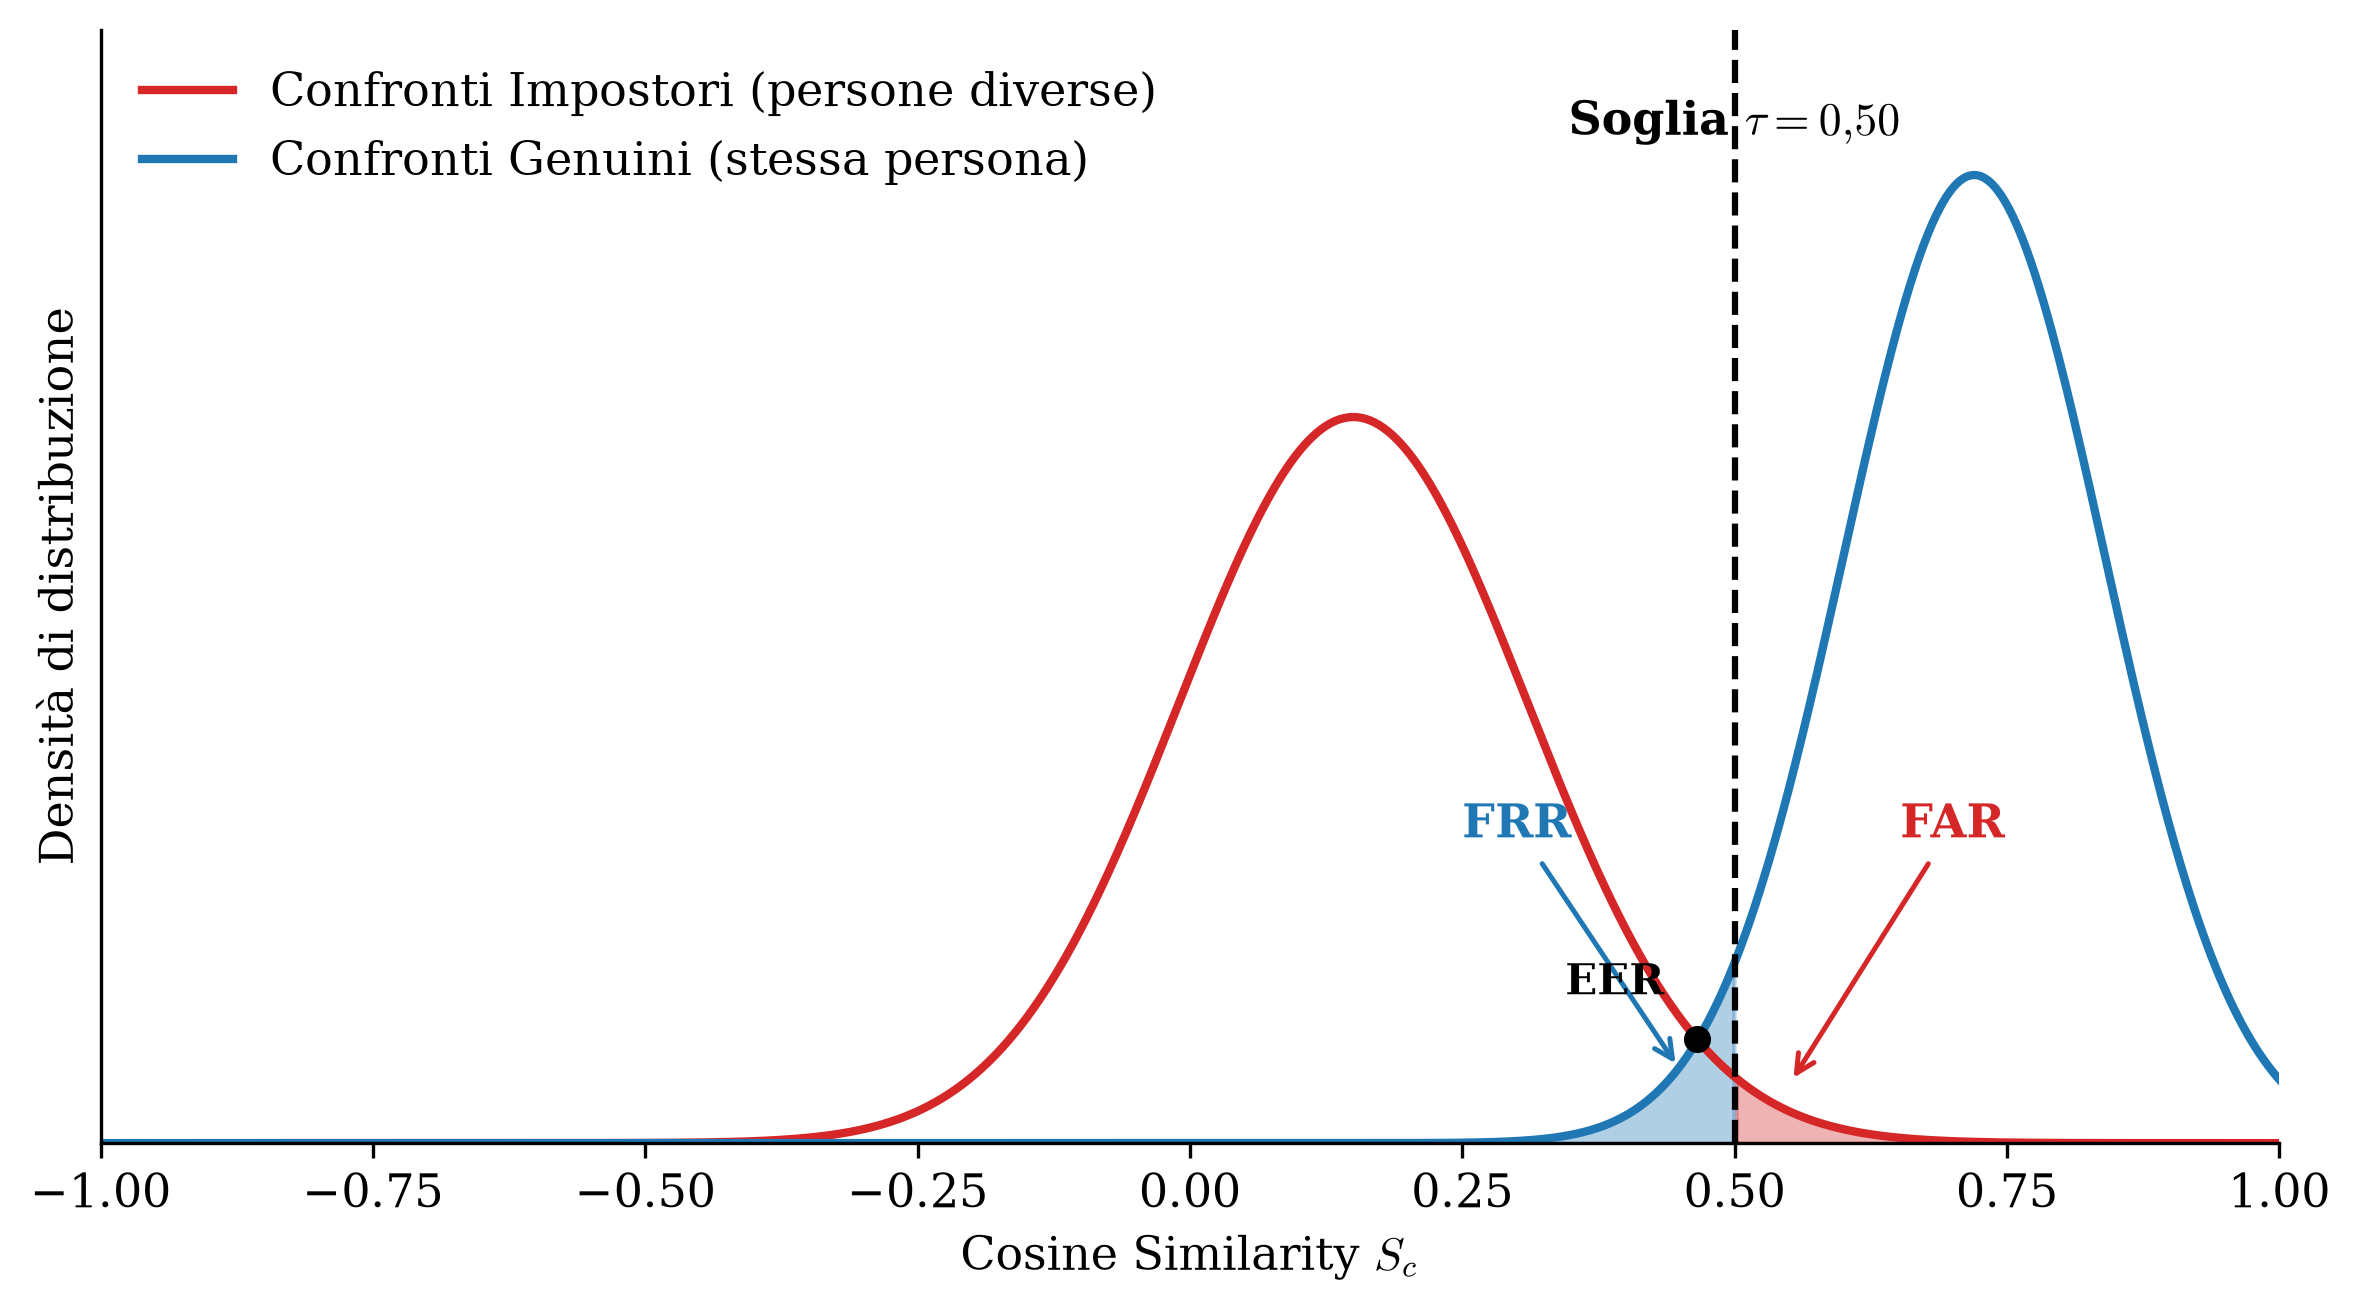
\includegraphics[width=0.8\linewidth]{images/impostore-genuino-frr-far.png}
    \caption[Distribuzione dei punteggi di \textit{Cosine Similarity} per confronti tra stesse persone e impostori]{Distribuzione dei punteggi di \textit{Cosine Similarity} ($S_c$) per confronti tra la stessa persona (genuini) e persone diverse (impostori). L'intersezione tra le due curve individua il punto di \gls{err}.}\label{fig:distribuzioni_far_frr}
\end{figure}

%===============================================

\section{Presentation Attack Detection (PAD) e Liveness Detection}\label{sec:padLiveness}
Nonostante l'elevata accuratezza garantita dai moderni modelli di \gls{frs} basati su \textit{deep embeddings}, i sistemi di autenticazione biometrica rimangono vulnerabili a un'ampia gamma di attacchi~\cite{azizFaceRecognitionBase2024}.
Ad esempio un malintenzionato può tentare di eludere il controllo biometrico riproducendo l'immagine di un utente legittimo, sotto forma di artefatto fisico o digitale davanti alla fotocamera. Tali minacce, note come \textit{\gls{pa}}, si manifestano comunemente come \textit{print attacks} (foto stampate) o \textit{replay attacks} (video o immagini riprodotte su schermi LCD).
Per normare la valutazione di sicurezza contro questi artefatti, lo standard internazionale \textbf{ISO/IEC 30107\-3} definisce le metriche prestazionali di riferimento per il \gls{pad}:
\begin{itemize}
    \item l'\textbf{\gls{apcer}} ovvero la percentuale di attacchi classificati erroneamente come legittimi;
    \item il \textbf{\gls{bpcer}} ovvero la percentuale di utenti legittimi classificati erroneamente come attacchi.
\end{itemize}
L'adozione di queste metriche consente di confrontare in modo oggettivo le prestazioni dei diversi algoritmi di \textit{liveness detection}~\cite{groupBiometricLivenessPresentation}.

Dal punto di vista della progettazione architetturale, le contromisure \gls{pad}, per verificare la \textbf{liveness} del soggetto, si suddividono in due macro-categorie:
\begin{itemize}
    \item \textbf{Approcci attivi} \textit{(challenge-response)}: richiedono una cooperazione esplicita da parte dell'utente, imponendo interazioni guidate come il movimento della testa, il battito delle ciglia volontario \textit{(blinking)} o la pronuncia di frasi casuali. Questi metodi sono più robusti contro gli attacchi \gls{pa}, ma possono risultare invasivi e creano barriere nella \gls{ux} del sistema;
    \item \textbf{Approcci passivi} \textit{(automatic/unobtrusive)}: operano in maniera trasparente e non intrusivo per l'utente. Si basano sull'analisi le micro-texture spaziali, i riflessi ottici e la coerenza cromatica di un breve flusso video, senza richiedere alcuna azione volontaria all'esterno. Questi metodi sono più \textit{user-friendly}, ma possono essere più vulnerabili a sofisticati attacchi di riproduzione~\cite{liSilentFaceAntiSpoofing2024}.
\end{itemize}
Nei metodi di verifica della \textit{liveness} passivi, si impiegano reti neurali convoluzionali ottimizzate per l'estrazione di feature a frequenza spaziale ridotta, ad esempio l'architettura \textit{MiniFASNet} derivata dal framework \textit{Silent-Face-Anti-Spoofing di Minivision-AI}. Infatti rappresenta la soluzione ideale per contesti operativi a \textbf{risorse limitate}: sono caratterizzate da un peso computazionale estremamente ridotto ($\sim 1\text{ MB}$) e dalla conversione dei pesi in formato \gls{onnx} Runtime. Riuscendo così, ad effettuare l'inferenza direttamente sui dispositivi \textit{edge} o client in modo efficiente, rilevando in modo efficiente gli artefatti ottici tipici di schermi e stampe fotografiche~\cite{liSilentFaceAntiSpoofing2024}.

Tuttavia, l'affidabilità del solo modulo di classificazione spaziale basato su singoli fotogrammi isolati, può risultare vulnerabile a variazioni di luminosità o a micro-artefatti di compressione del flusso video. Per garantire massima robustezza in un'applicazione reale, l'acquisizione non deve essere gestita come una transazione \textit{stateless} isolata, bensì come un processo continuo governato da una \textbf{macchina a stati finiti \gls{fsm}} integrata in una politica di campionamento a buffer temporale.
Durante la fase di acquisizione in tempo reale dalla fotocamera, il sistema raccoglie un buffer mobile di breve durata (composto tipicamente da 30 a 60 fotogrammi, pari a circa 2 secondi di stream video), calcolando iterativamente lo \textit{score} di \textit{liveness} per ogni fotogramma e scartando i frame affetti da \textit{motion blur} o scarsa nitidezza. Inoltre si tracciano temporalmente anche i 5 \textit{\gls{kbs}} durante il flusso video, per monitorare la varianza spaziale e rilevare la staticità innaturale di un \gls{pa}. La \gls{fsm} guida l'utente attraverso stati deterministici, transitando dallo stato di attesa del volto \textit{(Waiting Face)} alle fasi di analisi attiva in cui vengono accumulati i punteggi di confidenza e isolato il fotogramma più nitido e frontale. Solo qualora la media aritmetica dei punteggi degli \textit{score} dell'intero \textit{buffer} superi una soglia di sicurezza critica $\tau_{\text{liveness}}$, il sistema convalida la presenza biologica reale del soggetto ed effettua la ricerca nel database vettoriale. Al contrario, il rilevamento di uno score medio inferiore alla soglia $\tau_{\text{liveness}}$ o la presenza $M$ fotogrammi classificati come \textit{spoof} determina il rifiuto dell'autenticazione e la segnalazione di un potenziale attacco \gls{pa}~\cite{liSilentFaceAntiSpoofing2024}. Questa \textit{pipeline} è sintetizzata nel diagramma in Figura~\ref{fig:pipelineLiveness}.
\begin{figure}[H]
    \centering
    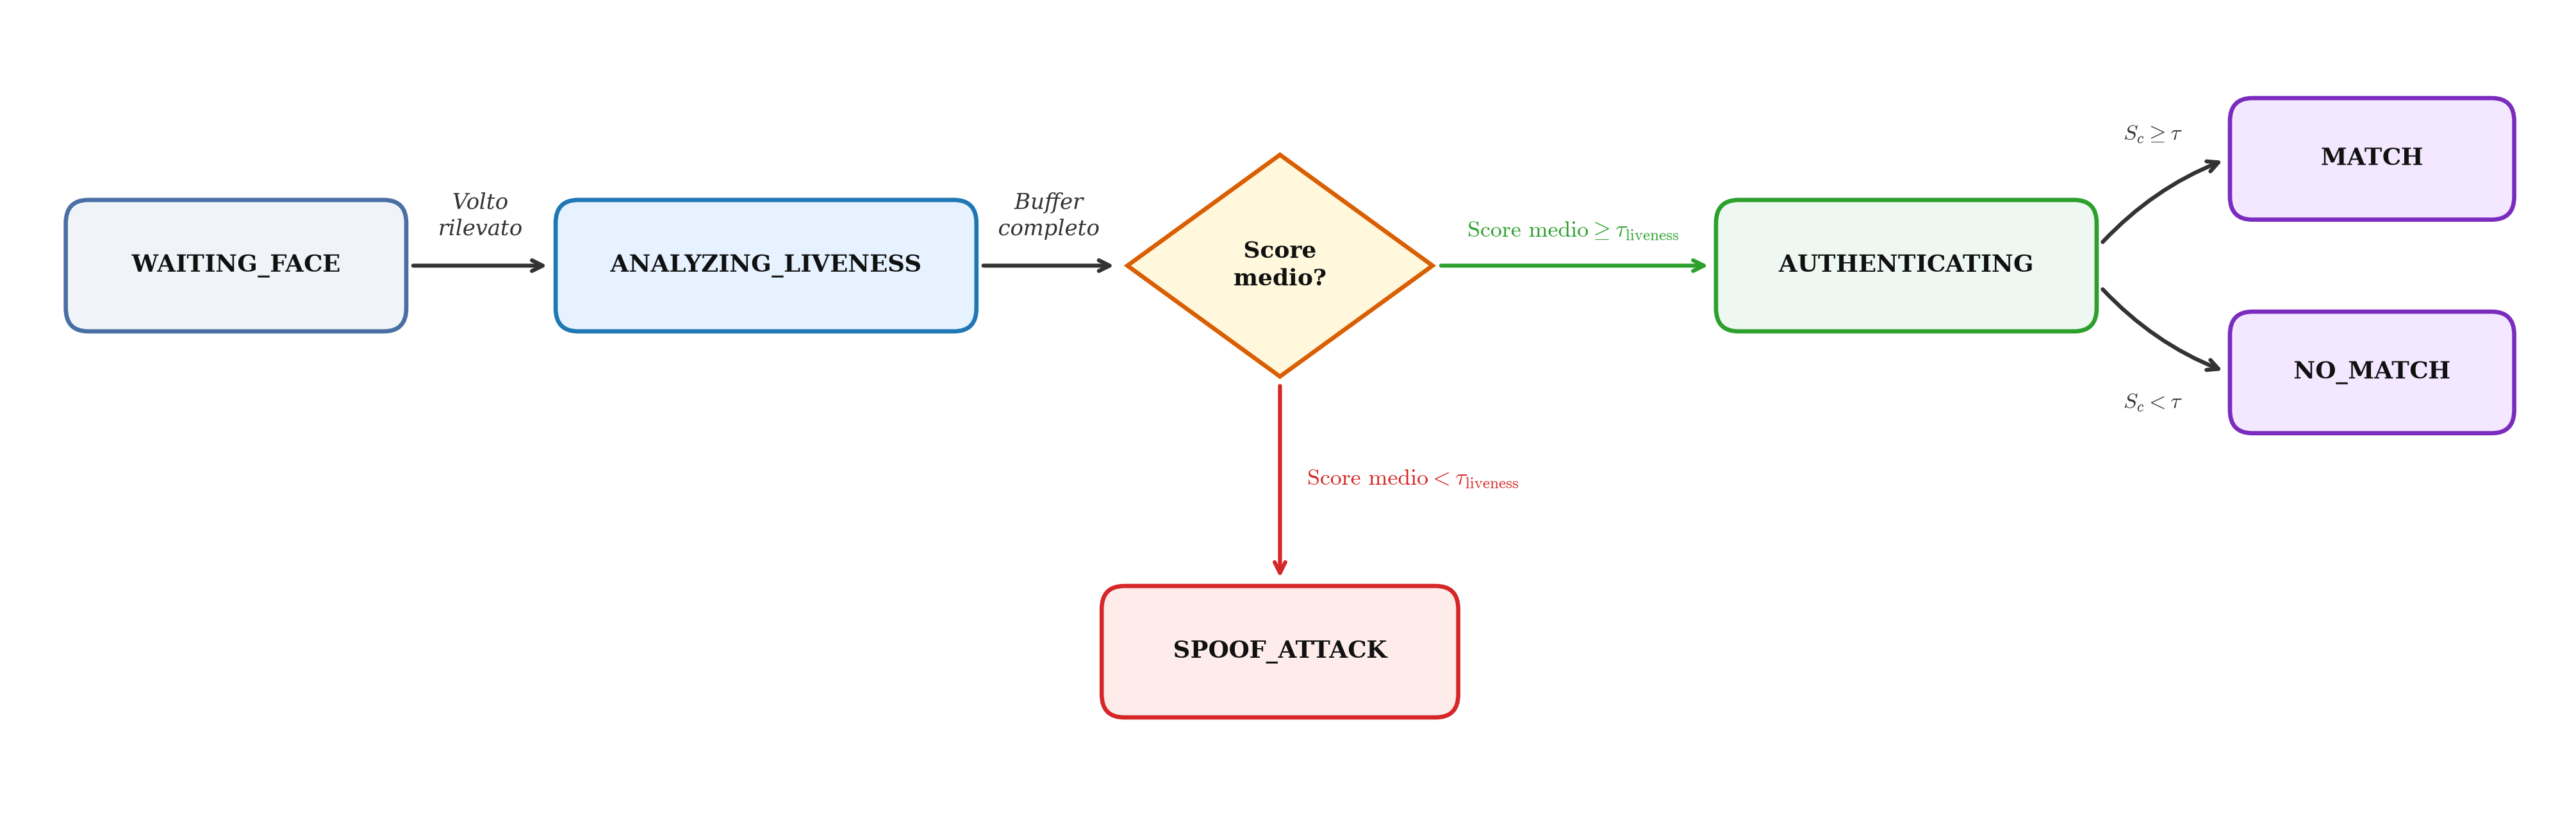
\includegraphics[width=1\linewidth]{images/pipeline-liveness.png}
    \caption{Diagramma di funzionamento della \gls{fsm} per la \textit{Liveness Detection} passiva e l'autenticazione biometrica.}\label{fig:pipelineLiveness}
\end{figure}

%===============================================

\section{Documenti d'identità e Cross-Domain Matching}
L'affidabiltà di un sistema di autenticazione biometrica remota basato su documenti d'identità fonda le proprie radici sulla rigorosa standardizzazione dei formati fisici e logici dei documenti stessi. A livello internazionale, l'\textbf{\gls{icao}} ha definito le specifiche tecniche per i documenti di viaggio, come passaporti e carte d'identità, nel documento \textit{Machine Readable Travel Documents (ICAO 9303)}~\cite{icao9303}.
Tra i formati definiti, lo standard specifica il formato \textbf{TD1} che corrisponde alle dimensioni tipiche di una carta di credito (85,6 mm × 53,98 mm) adottato per le \gls{cie} e le patenti di guida di paesi europei.
Il formato \textbf{TD1} prevede delle zone visive e delle zone leggibili a macchina come la \textit{\gls{mrz}} collocata sul retro del documento.
In particolare la sezione \textit{MRZ} contiene tre righe di testo di 30 caratteri con il font a spaziatura fissa \textit{OCR-B}. 
Essa viene elaborata con algoritmi di \gls{ocr} e riporta informazioni anagrafiche e biometriche del titolare, come il nome, la data di nascita, la nazionalità e il numero del documento, integrando anche un codice di controllo per validare l'integrità formale.
Inoltre, nei documenti dotati di chip a contatto o \textit{contactless} (come le \gls{cie}), la \textit{MRZ} funge da chiave di accesso per leggere i dati biometrici memorizzati nel chip~\cite{kelesRepublicTurkeyIdentity2020}.

In molti contesti applicativi, orientati alla massima fluiditità della \gls{ux}, l'interazione viene snellita limitando la cattura al solo lato anteriore del documento di identità. In tale modo si inibisce al sistema l'accesso diretto alla \gls{mrz} e al chip NFC, costringendo il \gls{frs} a estrarre il template biometrico di riferimento esclusivamente dalla fotografia \textit{(fototessera)} del volto stampata sul documento. 
Questa modalità operativa introduce una delle sfide più complesse nel campo della \textit{computer vision}: il \textbf{\textit{Cross-Domain Matching}}, evidenziate anche nella tabella~\ref{tab:crossDomainCriticita}. 
In questo scenario, il sistema deve confrontare due domini visivi profondamente eterogenei, acquisiti in condizioni ambientali e con qualità molto diverse tra loro: da un lato la fototessera presente sul documento d'identità, dall'altro l'immagine acquisita in diretta dalla fotocamera dell'utente.
Nello specifico, la foto del documento presenta spesso notevoli degradazioni visive dovute a:
\begin{itemize}
    \item inchiostri di stampa a bassa risoluzione;
    \item riflessi di luce e pattern olografici di sicurezza;
    \item artefatti da compressione JPEG (\textit{lossy});
    \item distorsioni geometriche legate all'inquadratura;
    \item differenze temporali dovute all'invecchiamento del soggetto (\textit{age-gap}).
\end{itemize}
Al contrario, lo scatto acquisito in tempo reale (\textit{live}) risente principalmente di fattori ambientali e comportamentali, quali variazioni di illuminazione, posa del volto ed espressione facciale.
Quindi si è notato che applicare direttamente un modello di \gls{frs} provoca un \textbf{drastico calo delle prestazioni}, facendo crollare il tasso di riconoscimento \gls{tar} a parità di falsi positivi \gls{far}, a causa della perdita di dettagli ad alta frequenza spaziale nell'immagine del documento~\cite{shiDocFaceMatchingID2018}.

\begin{table}[H]
    \centering
    \footnotesize
    %\begin{tabular}{c c c c}
    \begin{tabular*}{\textwidth}{@{\extracolsep{\fill}} >{\raggedright\arraybackslash}p{3.2cm} >{\raggedright\arraybackslash}p{4.8cm} >{\raggedright\arraybackslash}p{4.8cm} @{}}
        \hline
        \textbf{Criticità} & \textbf{Dominio Documentale} & \textbf{Dominio Live} \\
         & \textbf{[\gls{cie} / Passaporto]} & \textbf{[Webcam / Mobile]} \\
        \hline
        \textbf{Risoluzione Ottica} & Bassa (fototessera compressa o rasterizzata) & Elevata (sensore digitale in streaming) \\
        %\hline
        \textbf{Condizioni di Luce} & Statica, soggetta a riflessi superficiali olografici & Dinamica, variabile in base all'ambiente \\
        %\hline
        \textbf{Variabilità Temporale} & Presenza di \textit{age-gap} marcato (documento decennale) & Reale e sincrona al momento dell'autenticazione \\
        \hline
    %\end{tabular}
    \end{tabular*}
    \caption{Confronto delle caratteristiche e dei fattori di degrado tra il dominio documentale e il dominio live nel Cross-Domain Matching.}
    \label{tab:crossDomainCriticita}
\end{table}


Per mitigare questo problema, e garantire che il modulo di estrazione geometrica \textit{face alignment} operi su dati stabili, la pipeline di pre-elaborazione del sistema deve integrare \textbf{algoritmi di normalizzazione ottica e spaziale}.
Quando l'utente inquadra la carta d'identità tramite la fotocamera, il documento può presentare rotazioni sul piano, inclinazioni prospettiche o disuniformità di illuminazione dovute a riflessi speculari sulla superficie plastificata~\cite{yanezImageQualityAssessment2021a}.
Per correggerle si applica un modulo di individuazione dei confini del documento, che rileva i quattro vertici del rettangolo e calcola una \textbf{trasformazione prospettica} di rettifica \textit{warp perspective} per riallineare il documento a una griglia di riferimento.
Successivamente, si applica anche un algoritmo per contrastare la scarsa nitidezza e compressione tipica delle fototessere, come il \gls{clahe}: un \textbf{metodo di equalizzazione adattiva} dell'istogramma che opera su finestre locali dell'immagine anziché a livello globale. A differenza della normale equalizzazione, \gls{clahe} limita la amplificazione del rumore circostante imponendo una soglia massima, esaltando quindi i micro-dettagli della regione facciale (come i contorni degli occhi, del naso e della bocca)~\cite{rezaRealizationContrastLimited2004}.
Tutto ciò, rende il ritratto documentale geometricamente e cromaticamente compatibile con i fotogrammi live acquisiti dalla fotocamera, pronto per l'estrazione dei 5 keypoint biometrici e del calcolo dei vettori di embedding.

%===============================================

\section{Sicurezza biometrica e normative europee}\label{cap:1.4-normative}
L'integrazione di un sistema \gls{frs} in un'infrastruttura di autenticazione remota, espone l'intera pipeline biometrica a una superficie d'attacco ben più ampia dei soli attacchi \gls{pa} descritti nella Sezione~\ref{sec:padLiveness}.
In letteratura, la modellazione delle minacce (\textit{threat modeling}) lungo gli stadi della pipeline biometrica viene formalizzata con una \textbf{tassonomia di esposizione} e \textit{leakage} dei dati sensibili a sei livelli ($L1-L6$), come mostrato anche in Figura~\ref{fig:pipelineStadi-L1-L6}~\cite{sanzGoverningPrivacyPreservingFace2026}.
\begin{itemize}
    \item \textbf{Livello L1: \textit{Raw biometrics}}: esposizione dei fotogrammi grezzi acquisiti dalla fotocamera, contenenti informazioni biometriche sensibili e non anonimizzate;
    \item \textbf{Livello L2: \textit{Intermediate representations}}: intercettazione dei ritagli facciali normalizzati \textit{face crops} e dei \textit{keypoint biometrici}, che possono essere utilizzati per ricostruire il volto originale;
    \item \textbf{Livello L3: \textit{Embeddings and templates}}: compromissione dei vettori numerici di embedding $e \in \mathbb{R}^{512}$ che contengono informazioni biometriche sufficienti per identificare un individuo e possono essere utilizzati per attacchi di \textit{model inversion};
    \item \textbf{Livello L4: \textit{Model Parameters}}: accesso non autorizzato ai pesi $\theta$ della rete neurale, tra il volto acquisito e quello memorizzato nel database, che possono essere sfruttati per attacchi di \textit{model extraction} o \textit{membership inference};
    \item \textbf{Livello L5: \textit{Database e metadati}}: violazione dell'archivio centrale contenente gli embedding di riferimento e i metadati associati, che può portare a furto d'identità o profilazione non autorizzata;
    \item \textbf{Livello L6: \textit{Canali di comunicazione}}: attacchi sui canali di trasmissione dati, sulle API client-server o sulle connessioni cifrate, che possono consentire intercettazioni, \textit{replay} o \textit{man-in-the-middle}.
\end{itemize}
\begin{figure}[H]
    \centering
    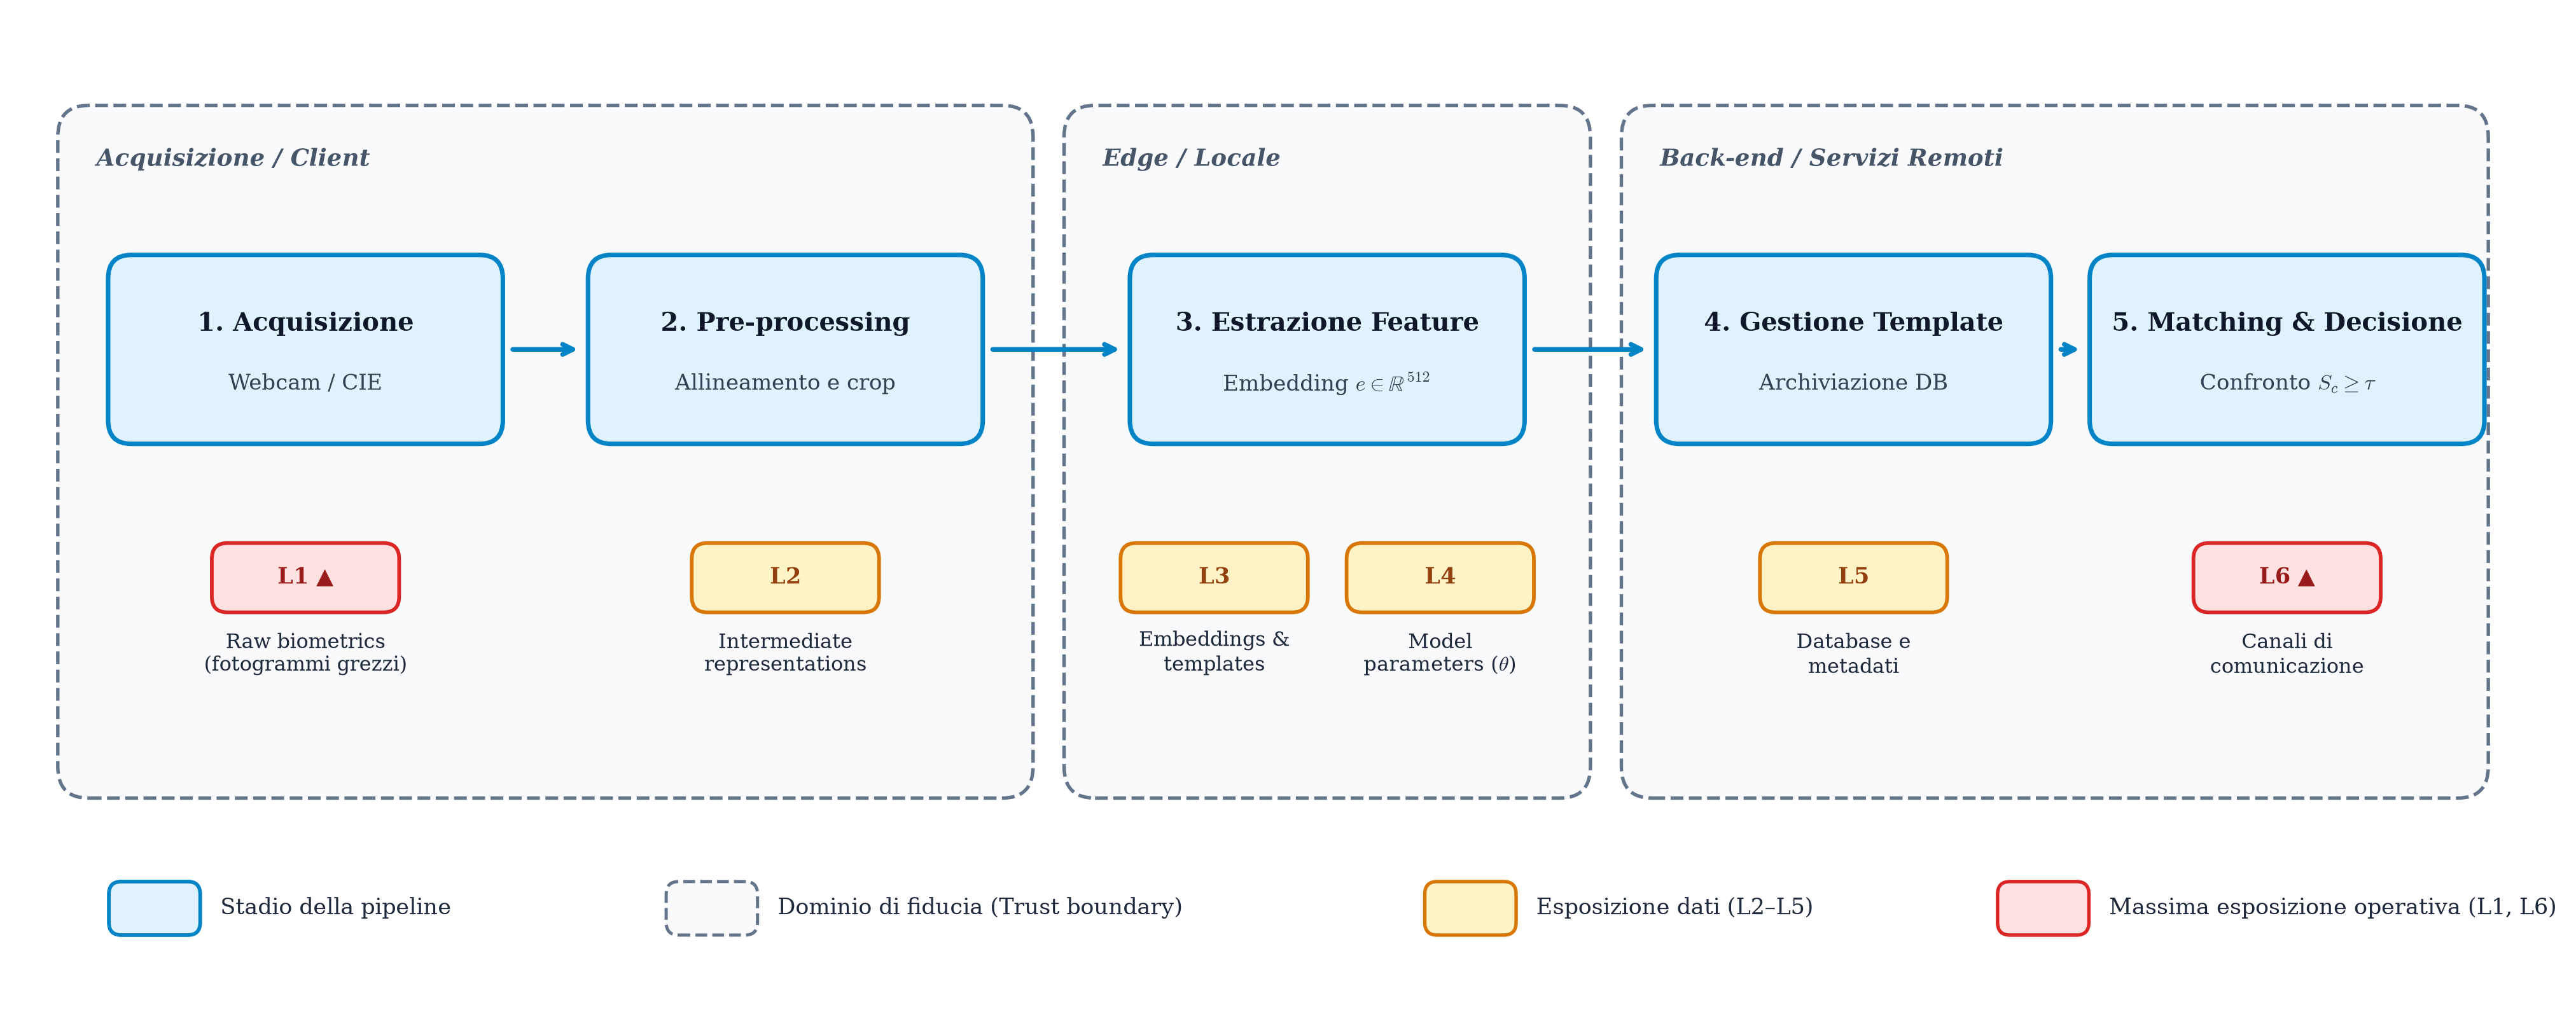
\includegraphics[width=\linewidth]{images/pipeline-stadiL1-L6.png}
    \caption[Architettura della pipeline di riconoscimento facciale e mappatura dei livelli di esposizione dei dati sensibili]{Architettura a cinque stadi della pipeline di riconoscimento facciale e mappatura dei sei livelli di esposizione dei dati sensibili ($L1\text{--}L6$) lungo i diversi domini operativi}\label{fig:pipelineStadi-L1-L6}
\end{figure}
I moduli \textit{\gls{pad}} presidiano l'integrità fisica a monte del sensore ottico, invece i livelli $L1-L6$ risultano particolarmente critici rispetto agli \textbf{attacchi di iniezione digitale} (\textit{digital injection attacks}) e alle \textbf{minacce di compromissione dei dati biometrici}~\cite{groupBiometricLivenessPresentation}.
In uno scenario di iniezione, l'attaccante aggira completamente la fotocamera fisica iniettando nel flusso di cattura un video pre-registrato, manipolato o generato sinteticamente (\textit{deepfake}) mediante l'uso di driver di fotocamere virtuali (\textit{virtual cameras}), emulatori software o la manomissione del payload trasmesso verso il server~\cite{groupBiometricLivenessPresentation}.
In questo modo il flusso video iniettato non subisce la degradazione ottica di una lente reale, nè presenta gli artefatti di ricattura tipici di uno schermo LCD (come i pattern di moiré o i riflessi speculari), risultando quindi più difficile da rilevare per i moduli \gls{pad} di \textit{liveness detection}.
Per questa ragione la specifica tecnica europea \textbf{CEN/TS 18099:2024} (\textit{Biometric data injection attack detection}) separa formalmente le minacce di \textit{presentation attack} da quelle di \textit{digital injection attack}, definendo contromisure architetturali quali:
\begin{itemize}
    \item \textbf{il controllo dell'integrità} del canale di acquisizione video, mediante l'uso di firme digitali e \textit{hashing} dei fotogrammi;
    \item \textbf{la validazione crittografica} delle sessioni temporizzate
    \item \textbf{l'impiego di vincoli temporali} sulle transazioni di autenticazione, per prevenire attacchi di \textit{replay} e \textit{man-in-the-middle};
    \item \textbf{l'analisi della coerenza} spazio-temporale dei fotogrammi acquisiti.
\end{itemize}

Un'altra minaccia riguarda la vulnerabilità agli attacchi di ricostruzione noti come \textbf{\textit{model inversion}} e \textit{feature extraction}, che possono compromettere i livelli $L3-L5$~\cite{otroshishahrezaBenchmarkingCancelableBiometrics2022,sanzGoverningPrivacyPreservingFace2026}.
È importante sottolineare, che un \textit{deep face embedding} $e \in \mathbb{R}^{512}$ \textbf{non equivale} a un'impronta crittografica unidirezionale (come un hash \textit{SHA-256}). 
Questo poichè due acquisizioni successive del medesimo volto presentano inevitabilmente piccole variazioni dovute al rumore del sensore, all'illuminazione e alla posa. Quindi i rispettivi vettori di embedding $e_i$ e $e_j$ non saranno \textbf{mai identici} bit a bit.
L'applicazione di una funzione di hash crittografica standard, a causa dell'\textit{effetto valanga}, produrrebbe stringhe binarie totalmente incorrelate, rendendo impossibile il confronto tramite \textit{Cosine Similarity}~\cite{otroshishahrezaBenchmarkingCancelableBiometrics2022}.
Tuttavia, recenti studi sulla sicurezza biometrica hanno dimostrato che un attaccante in possesso dei vettori di embedding in chiaro (ad esempio in seguito a un \textit{data breach}) può addestrare una rete neurale generativa o un decodificatore inverso per \textbf{ricostruire un'approssimazione fotorealistica} del volto originale a partire dalle sole 512 componenti, arrivando ad ingannare lo stesso sistema biometrico~\cite{otroshishahrezaBenchmarkingCancelableBiometrics2022}.
A differenza di una password alfanumerica, che può essere sostituita istantaneamente in caso di furto, le caratteristiche biometriche fisiologiche sono intrinsecamente legate all'individuo e \textbf{non possono essere revocate}.
Per questo motivo, lo standard internazionale \textbf{ISO/IEC 24745} stabilisce che i meccanismi di \textbf{\textit{Biometric Template Protection} (BTP)} e di \textbf{biometria cancellabile (\textit{Cancelable Biometrics}, CB)} debbano soddisfare quattro proprietà fondamentali~\cite{otroshishahrezaBenchmarkingCancelableBiometrics2022}:
\begin{enumerate}
    \item \textbf{Irreversibilità}: deve risultare computazionalmente infattibile ricostruire l'embedding originale $e$ a partire dal template protetto, garantendo una indipendenza $MI(X,Y)\sim0$ prossima allo zero tra il template originale $X$ e quello trasformato $Y$;
    \item \textbf{Revocabilità}: in caso di compromissione del template protetto, deve essere possibile generare un nuovo template indipendente $Y'$ a partire dallo stesso embedding originale $e$, annullando il precedente, modificando una chiave o un seme associato all'utente;
    \item \textbf{Non correlabilità}: i template protetti $Y$ e $Y'$ generati a partire dallo stesso embedding originale $e$ non devono essere correlabili tra loro, impedendo attacchi di \textit{cross-matching} tra database diversi, prevenendo il tracciamento incrociato dell'utente;
    \item \textbf{Preservazione delle prestazioni}: la trasformazione matematica non deve degradare l'accuratezza discriminativa del sistema in termini di \gls{far}, \gls{frr} e \gls{err}, mantenendo un tasso di riconoscimento \gls{tar} comparabile a quello ottenuto con gli embedding originali.
\end{enumerate}
Tra gli schemi di \textit{Cancelable Biometrics} più consolidati e diffusi per la protezione dei dati biometrici, figura il \textbf{BioHashing}~\cite{otroshishahrezaBenchmarkingCancelableBiometrics2022}.
Dato il vettore biometrico estratto $e \in \mathbb{R}^{512}$ e un token segreto (\textit{seed crittografico} $K$) specifico dell'utente, l'algoritmo genera una matrice pseudo-casuale a partire da $K$, applicando il procedimento di ortonormalizzazione di \textit{Gram-Schmidt}. In questo modo si ottiene una base di $m$ vettori ortonormali $b_i \in \mathbb{R}^{512}$ (con $i \in \{1, \dots, m\}$ e $m \le 512$), utili a garantire che le proiezioni successive non siano correlate tra loro.
Quindi il template protetto $c = [c_1, c_2, \dots, c_m] \in {\left\{0, 1\right\}}^m$ viene generato proiettando l'embedding originale $e$ su ciascun vettore della base ortonormale $b_i$ e applicando una soglia binaria $\tau_{\text{biohash}}$ al risultato,come mostrato nell'Equazione~\eqref{eq:biohashing}~\cite{otroshishahrezaBenchmarkingCancelableBiometrics2022}:
\begin{equation}
    \label{eq:biohashing}
    c_i = \begin{cases} 1 & \text{se } \langle e, b_i \rangle \ge \tau_{\text{bh}} \\ 0 & \text{se } \langle e, b_i \rangle < \tau_{\text{bh}} \end{cases} \quad \forall i \in \{1, \dots, m\}
\end{equation}
dove $\langle e, b_i \rangle$ indica il prodotto scalare tra l'embedding e l'$i$-esimo vettore della base, mentre $\tau_{\text{bh}}$ è la soglia di binarizzazione (tipicamente fissata a $0$). 
Questo passaggio trasforma il vettore numerico originale in una stringa binaria non invertibile: anche in caso di furto del template $c$ protetto, è computazionalmente impossibile risalire all'embedding originale $e$ senza la conoscenza del token segreto $K$. Mentre se viene compromesso il \textit{seed} $K$ è sufficiente revocarlo e generarne uno nuovo. 
Affinché la protezione sia efficace, però, contro eventuali violazioni del database (\textit{data breach}), la sicurezza dello schema si fonda sulla \textbf{separazione architetturale} tra il template protetto $c$ e il token segreto $K$. 
Ovvero il template binario risiede sul server, mentre il \textit{seed} $K$ deve essere custodito separatamente: ad esempio localmente sul dispositivo dell'utente (in un'area protetta hardware), derivato da una password tramite funzioni di derivazione crittografica, oppure gestito in un servizio isolato di gestione delle chiavi (\textit{\gls{kms}}).
\\In fase di verifica, il confronto tra due template binari avviene tramite la \textbf{distanza di Hamming}, calcolata come il numero di bit differenti tra i due vettori binari, normalizzata rispetto alla \textit{cosine similarity}~\cite{otroshishahrezaBenchmarkingCancelableBiometrics2022}.
In letteratura esistono anche soluzioni alternative, tra cui l'\textit{Index-of-Maximum (IoM) hashing}, l'\textit{MLP-Hashing} e la \textbf{Crittografia Omomorfica (\textit{Homomorphic Encryption}, HE)}~\cite{otroshishahrezaBenchmarkingCancelableBiometrics2022}.
Quest'ultima offre garanzie di sicurezza molto elevate, poichè permette al server di calcolare la distanza direttamente sui vettori cifrati senza mai doverli decifrare (mitigando i rischi ai livelli $L3$ e $L5$), ma introduce un pesante \textit{overhead} computazionale e richiede un'infrastruttura cloud con GPU dedicate per l'inferenza in tempo reale, rendendolo poco adatto a sistemi di autenticazione interattivi in tempo reale~\cite{otroshishahrezaBenchmarkingCancelableBiometrics2022}.
Nella Tabella~\ref{tab:tassonomiaLeakagePPFR} è riportata una sintesi della tassonomia di esposizione biometrica lungo la pipeline di riconoscimento, con le relative contromisure tecniche di \textit{Privacy-Preserving Face Recognition} (\textit{PPFR})~\cite{sanzGoverningPrivacyPreservingFace2026,otroshishahrezaBenchmarkingCancelableBiometrics2022,groupBiometricLivenessPresentation}.

\begin{table}[H]
    \centering
    \footnotesize
    %\begin{tabular}{c c c c}
    \begin{tabular*}{\textwidth}{@{\extracolsep{\fill}} c l p{4.6cm} p{4.3cm} @{}}
        \hline
        \textbf{Livello} & \textbf{Stadio Pipeline} & \textbf{Artefatto Esposto\newline e Minaccia} & \textbf{Contromisura Tecnica} \\
        \hline
        \textbf{L1} & Acquisizione & Immagini grezze CIE e frame video (\textit{Spoofing}, \textit{Injection Attacks}) & \gls{pad} passivo (\textit{MiniFASNet}), \textit{Zero-Disk Retention}, controllo canale \\
        %\hline
        \textbf{L2} & Pre-processing & \textit{Face crops} $112 \times 112$ e mappe di attivazione intermedie & Elaborazione in memoria volatile (RAM), \textit{Edge pre-processing} \\
        %\hline
        \textbf{L3} & Estrazione Feature & Embedding $e \in \mathbb{R}^{512}$ (\textit{Template Inversion Attack}) & \textit{Cancelable Biometrics} (\textit{BioHashing}), \textit{Template Protection} \\
        %\hline
        \textbf{L4} & Modello Neurale & Pesi $\theta$ della rete (\textit{Model Extraction}, \textit{Membership Inference}) & Esecuzione isolata su backend o \textit{Trusted Execution Environment} \\
        %\hline
        \textbf{L5} & Database & Archivio vettoriale e metadati (\textit{Data Breach}, \textit{Linkage Attack}) & Minimizzazione dei campi, cifratura \textit{at-rest}, disaccoppiamento ID \\
        %\hline
        \textbf{L6} & Comunicazione & Payload di rete, API REST e stream WebSocket (\textit{MitM}, \textit{Replay}) & Cifratura \textit{in-transit} (HTTPS/TLS, WSS), token JWT a scadenza breve \\
        \hline
    %\end{tabular}
    \end{tabular*}
    \caption[Tassonomia di esposizione biometrica lungo la pipeline]{Tassonomia di esposizione biometrica (L1--L6) lungo la pipeline di riconoscimento e relative contromisure di \gls{ppfr}~\cite{sanzGoverningPrivacyPreservingFace2026,otroshishahrezaBenchmarkingCancelableBiometrics2022,groupBiometricLivenessPresentation}.}\label{tab:tassonomiaLeakagePPFR}
\end{table}

La scelta delle contromisure di sicurezza lungo la tassonomia $L1-L6$ è vincolata al paradigma architetturale adottato. Si contrappongono due approcci principali: l'architettura \textbf{Server/Cloud Computing} (elaborazione centralizzata) e l'architettura \textbf{Edge Computing} (elaborazione sul dispositivo client). Il tutto nel rigoroso quadro normativo europeo delineato dal \textbf{\gls{gdpr}} e dal \textbf{AI Act}~\cite{sanzGoverningPrivacyPreservingFace2026}.
\begin{itemize}
    \item Ai sensi dell'\textbf{Articolo 9 del \gls{gdpr}}, i dati biometrici intesi a identificare in modo univoco una persona fisica costituiscono \textit{categorie particolari di dati personali} ovvero i \textbf{dati sensibili}, il cui trattamento è vietato salvo consenso esplicito dell'interessato e adozione di garanzie tecniche adeguate~\cite{REGOLAMENTOUE2016}.
    \item Inoltre l'\textbf{Articolo 5} e l'\textbf{Articolo 25} del \gls{gdpr} impongono i principi cardine di \textit{data minimization}, \textit{purpose limitation}, \textit{privacy by design} e \textit{privacy by default}, che richiedono l'adozione di misure tecniche e organizzative per garantire la protezione dei dati personali fin dalla progettazione del sistema, minimizzando la raccolta e il trattamento dei dati sensibili~\cite{REGOLAMENTOUE2016}.
    \item Parallelamente, l'\textbf{AI Act} europeo classifica i sistemi di riconoscimento facciale \gls{frs} come \textit{high-risk AI systems} (sistemi ad alto rischio), imponendo requisiti stringenti di robustezza contro i tentativi di manipolazione (come \textit{spoofing} e \textit{injection}), tracciabilità, supervisione umana e la trasparenza degli algoritmi, con l'obbligo di valutazioni d'impatto sulla protezione dei dati (\textit{DPIA}) e la conformità alle norme etiche e legali~\cite{sanzGoverningPrivacyPreservingFace2026}.
\end{itemize}
Dal punto di vista ingegneristico, un architettura puramente \textit{Edge-only}, in cui il rilevamento facciale, il \gls{pad} e il matching avvengono \textbf{interamente sul dispositivo} dell'utente, massimizza la tutela della privacy ai livelli $L1$ e $L6$, poichè nessun dato grezzo attraversa la rete. Tuttavia, si scontra con i limiti computazionali dei dispositivi mobili (che impediscono l'esecuzione di \textit{backbone} pesanti come \texttt{buffalo\_l} per l'estrazione da documenti degradati). Inoltre espone i pesi del modello al livello $L4$ e rende impraticabile una gestione multi-utente centralizzata (1
:N)~\cite{sanzGoverningPrivacyPreservingFace2026}.
Di contro, un'architettura puramente centralizzata garantisce \textbf{prestazioni e scalabilità} elevate, ma amplifica il rischio normativo e di superficie d'attacco qualora conservi su disco le immagini dei documenti o i flussi video~\cite{sanzGoverningPrivacyPreservingFace2026}.
Per superare questo disallineamento strutturale tra fattibilità operativa, sicurezza informatica e conformità legale, il sistema sviluppato in questa tesi adotta un'architettura ibrida fondata sui principi di \textbf{Privacy By Design} e \textbf{Zero Disk Retention}: i dati biometrici grezzi acquisiti dal client (come la scansione della \gls{cie} e i fotogrammi della webcam ai livelli $L1-L2$) vengono elaborati dal backend esclusivamente in memoria volatile (RAM) per pochi millisecondi, necessari all'inferenza su \textit{\gls{onnx} Runtime} e all'estrazione del vettore matematico. In seguito vengono \textbf{distrutti istantaneamente} senza mai essere scritti sul file system o nel database. In questo modo, la persistenza sul database vettoriale viene circoscritta alla sola rappresentazione numerica astratta associata all'identificativo utente, coniugando latenze da tempo reale con il pieno rispetto del principio di minimizzazione descritto in precedenza.
% Threat model e Injection Attacks; Model Inversion e BioHashing; Architetture Server vs Edge AI e conformità GDPR/AI Act
% 6pp